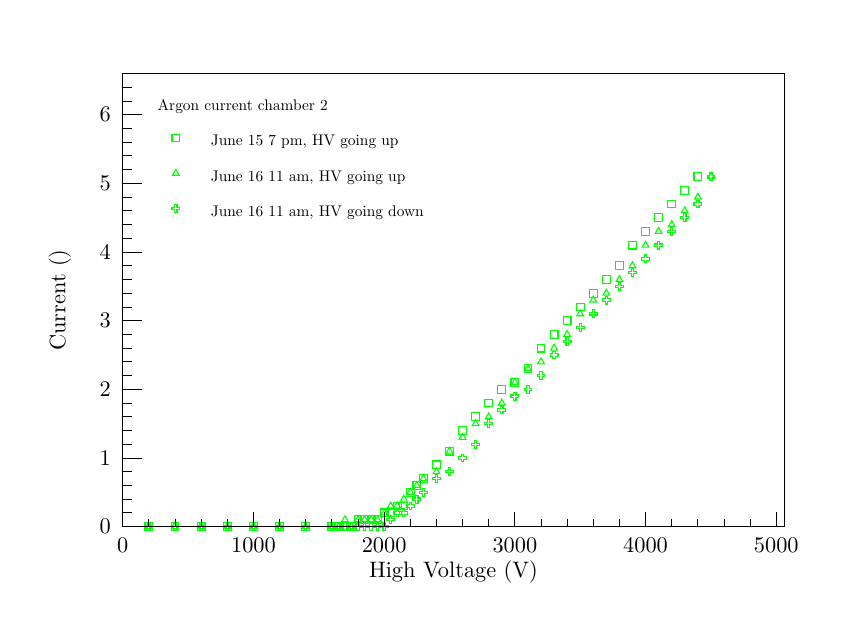
\begin{tikzpicture}
\pgfdeclareplotmark{cross} {
\pgfpathmoveto{\pgfpoint{-0.3\pgfplotmarksize}{\pgfplotmarksize}}
\pgfpathlineto{\pgfpoint{+0.3\pgfplotmarksize}{\pgfplotmarksize}}
\pgfpathlineto{\pgfpoint{+0.3\pgfplotmarksize}{0.3\pgfplotmarksize}}
\pgfpathlineto{\pgfpoint{+1\pgfplotmarksize}{0.3\pgfplotmarksize}}
\pgfpathlineto{\pgfpoint{+1\pgfplotmarksize}{-0.3\pgfplotmarksize}}
\pgfpathlineto{\pgfpoint{+0.3\pgfplotmarksize}{-0.3\pgfplotmarksize}}
\pgfpathlineto{\pgfpoint{+0.3\pgfplotmarksize}{-1.\pgfplotmarksize}}
\pgfpathlineto{\pgfpoint{-0.3\pgfplotmarksize}{-1.\pgfplotmarksize}}
\pgfpathlineto{\pgfpoint{-0.3\pgfplotmarksize}{-0.3\pgfplotmarksize}}
\pgfpathlineto{\pgfpoint{-1.\pgfplotmarksize}{-0.3\pgfplotmarksize}}
\pgfpathlineto{\pgfpoint{-1.\pgfplotmarksize}{0.3\pgfplotmarksize}}
\pgfpathlineto{\pgfpoint{-0.3\pgfplotmarksize}{0.3\pgfplotmarksize}}
\pgfpathclose
\pgfusepathqstroke
}
\pgfdeclareplotmark{cross*} {
\pgfpathmoveto{\pgfpoint{-0.3\pgfplotmarksize}{\pgfplotmarksize}}
\pgfpathlineto{\pgfpoint{+0.3\pgfplotmarksize}{\pgfplotmarksize}}
\pgfpathlineto{\pgfpoint{+0.3\pgfplotmarksize}{0.3\pgfplotmarksize}}
\pgfpathlineto{\pgfpoint{+1\pgfplotmarksize}{0.3\pgfplotmarksize}}
\pgfpathlineto{\pgfpoint{+1\pgfplotmarksize}{-0.3\pgfplotmarksize}}
\pgfpathlineto{\pgfpoint{+0.3\pgfplotmarksize}{-0.3\pgfplotmarksize}}
\pgfpathlineto{\pgfpoint{+0.3\pgfplotmarksize}{-1.\pgfplotmarksize}}
\pgfpathlineto{\pgfpoint{-0.3\pgfplotmarksize}{-1.\pgfplotmarksize}}
\pgfpathlineto{\pgfpoint{-0.3\pgfplotmarksize}{-0.3\pgfplotmarksize}}
\pgfpathlineto{\pgfpoint{-1.\pgfplotmarksize}{-0.3\pgfplotmarksize}}
\pgfpathlineto{\pgfpoint{-1.\pgfplotmarksize}{0.3\pgfplotmarksize}}
\pgfpathlineto{\pgfpoint{-0.3\pgfplotmarksize}{0.3\pgfplotmarksize}}
\pgfpathclose
\pgfusepathqfillstroke
}
\pgfdeclareplotmark{newstar} {
\pgfpathmoveto{\pgfqpoint{0pt}{\pgfplotmarksize}}
\pgfpathlineto{\pgfqpointpolar{44}{0.5\pgfplotmarksize}}
\pgfpathlineto{\pgfqpointpolar{18}{\pgfplotmarksize}}
\pgfpathlineto{\pgfqpointpolar{-20}{0.5\pgfplotmarksize}}
\pgfpathlineto{\pgfqpointpolar{-54}{\pgfplotmarksize}}
\pgfpathlineto{\pgfqpointpolar{-90}{0.5\pgfplotmarksize}}
\pgfpathlineto{\pgfqpointpolar{234}{\pgfplotmarksize}}
\pgfpathlineto{\pgfqpointpolar{198}{0.5\pgfplotmarksize}}
\pgfpathlineto{\pgfqpointpolar{162}{\pgfplotmarksize}}
\pgfpathlineto{\pgfqpointpolar{134}{0.5\pgfplotmarksize}}
\pgfpathclose
\pgfusepathqstroke
}
\pgfdeclareplotmark{newstar*} {
\pgfpathmoveto{\pgfqpoint{0pt}{\pgfplotmarksize}}
\pgfpathlineto{\pgfqpointpolar{44}{0.5\pgfplotmarksize}}
\pgfpathlineto{\pgfqpointpolar{18}{\pgfplotmarksize}}
\pgfpathlineto{\pgfqpointpolar{-20}{0.5\pgfplotmarksize}}
\pgfpathlineto{\pgfqpointpolar{-54}{\pgfplotmarksize}}
\pgfpathlineto{\pgfqpointpolar{-90}{0.5\pgfplotmarksize}}
\pgfpathlineto{\pgfqpointpolar{234}{\pgfplotmarksize}}
\pgfpathlineto{\pgfqpointpolar{198}{0.5\pgfplotmarksize}}
\pgfpathlineto{\pgfqpointpolar{162}{\pgfplotmarksize}}
\pgfpathlineto{\pgfqpointpolar{134}{0.5\pgfplotmarksize}}
\pgfpathclose
\pgfusepathqfillstroke
}
\definecolor{c}{rgb}{1,1,1};
\draw [color=c, fill=c] (0,0) rectangle (10,7.19298);
\definecolor{c}{rgb}{0,0,0};
\draw [c,line width=0.3] (1.2,0.863158) -- (1.2,6.61754) -- (9.6,6.61754) -- (9.6,0.863158) -- (1.2,0.863158);
\draw [c,line width=0.3] (1.2,0.863158) -- (1.2,6.61754) -- (9.6,6.61754) -- (9.6,0.863158) -- (1.2,0.863158);
\draw [c,line width=0.3] (1.2,0.863158) -- (1.2,6.61754) -- (9.6,6.61754) -- (9.6,0.863158) -- (1.2,0.863158);
\draw [c,line width=0.3] (1.2,0.863158) -- (1.2,6.61754) -- (9.6,6.61754) -- (9.6,0.863158) -- (1.2,0.863158);
\draw [c,line width=0.3] (1.2,0.863158) -- (9.6,0.863158);
\draw [c,line width=0.3] (1.2,1.04442) -- (1.2,0.863158);
\draw [c,line width=0.3] (1.53202,0.953789) -- (1.53202,0.863158);
\draw [c,line width=0.3] (1.86403,0.953789) -- (1.86403,0.863158);
\draw [c,line width=0.3] (2.19605,0.953789) -- (2.19605,0.863158);
\draw [c,line width=0.3] (2.52806,0.953789) -- (2.52806,0.863158);
\draw [c,line width=0.3] (2.86008,1.04442) -- (2.86008,0.863158);
\draw [c,line width=0.3] (3.19209,0.953789) -- (3.19209,0.863158);
\draw [c,line width=0.3] (3.52411,0.953789) -- (3.52411,0.863158);
\draw [c,line width=0.3] (3.85613,0.953789) -- (3.85613,0.863158);
\draw [c,line width=0.3] (4.18814,0.953789) -- (4.18814,0.863158);
\draw [c,line width=0.3] (4.52016,1.04442) -- (4.52016,0.863158);
\draw [c,line width=0.3] (4.85217,0.953789) -- (4.85217,0.863158);
\draw [c,line width=0.3] (5.18419,0.953789) -- (5.18419,0.863158);
\draw [c,line width=0.3] (5.51621,0.953789) -- (5.51621,0.863158);
\draw [c,line width=0.3] (5.84822,0.953789) -- (5.84822,0.863158);
\draw [c,line width=0.3] (6.18024,1.04442) -- (6.18024,0.863158);
\draw [c,line width=0.3] (6.51225,0.953789) -- (6.51225,0.863158);
\draw [c,line width=0.3] (6.84427,0.953789) -- (6.84427,0.863158);
\draw [c,line width=0.3] (7.17628,0.953789) -- (7.17628,0.863158);
\draw [c,line width=0.3] (7.5083,0.953789) -- (7.5083,0.863158);
\draw [c,line width=0.3] (7.84032,1.04442) -- (7.84032,0.863158);
\draw [c,line width=0.3] (8.17233,0.953789) -- (8.17233,0.863158);
\draw [c,line width=0.3] (8.50435,0.953789) -- (8.50435,0.863158);
\draw [c,line width=0.3] (8.83636,0.953789) -- (8.83636,0.863158);
\draw [c,line width=0.3] (9.16838,0.953789) -- (9.16838,0.863158);
\draw [c,line width=0.3] (9.50039,1.04442) -- (9.50039,0.863158);
\draw [c,line width=0.3] (9.50039,1.04442) -- (9.50039,0.863158);
\draw [anchor=base] (1.2,0.539474) node[scale=0.807119, color=c, rotate=0]{0};
\draw [anchor=base] (2.86008,0.539474) node[scale=0.807119, color=c, rotate=0]{1000};
\draw [anchor=base] (4.52016,0.539474) node[scale=0.807119, color=c, rotate=0]{2000};
\draw [anchor=base] (6.18024,0.539474) node[scale=0.807119, color=c, rotate=0]{3000};
\draw [anchor=base] (7.84032,0.539474) node[scale=0.807119, color=c, rotate=0]{4000};
\draw [anchor=base] (9.50039,0.539474) node[scale=0.807119, color=c, rotate=0]{5000};
\draw (5.4,0.287719) node[scale=0.807119, color=c, rotate=0]{High Voltage (\si{V})};
\draw [c,line width=0.3] (1.2,0.863158) -- (1.2,6.61754);
\draw [c,line width=0.3] (1.44,0.863158) -- (1.2,0.863158);
\draw [c,line width=0.3] (1.32,1.03753) -- (1.2,1.03753);
\draw [c,line width=0.3] (1.32,1.21191) -- (1.2,1.21191);
\draw [c,line width=0.3] (1.32,1.38628) -- (1.2,1.38628);
\draw [c,line width=0.3] (1.32,1.56066) -- (1.2,1.56066);
\draw [c,line width=0.3] (1.44,1.73503) -- (1.2,1.73503);
\draw [c,line width=0.3] (1.32,1.90941) -- (1.2,1.90941);
\draw [c,line width=0.3] (1.32,2.08379) -- (1.2,2.08379);
\draw [c,line width=0.3] (1.32,2.25816) -- (1.2,2.25816);
\draw [c,line width=0.3] (1.32,2.43254) -- (1.2,2.43254);
\draw [c,line width=0.3] (1.44,2.60691) -- (1.2,2.60691);
\draw [c,line width=0.3] (1.32,2.78129) -- (1.2,2.78129);
\draw [c,line width=0.3] (1.32,2.95566) -- (1.2,2.95566);
\draw [c,line width=0.3] (1.32,3.13004) -- (1.2,3.13004);
\draw [c,line width=0.3] (1.32,3.30441) -- (1.2,3.30441);
\draw [c,line width=0.3] (1.44,3.47879) -- (1.2,3.47879);
\draw [c,line width=0.3] (1.32,3.65316) -- (1.2,3.65316);
\draw [c,line width=0.3] (1.32,3.82754) -- (1.2,3.82754);
\draw [c,line width=0.3] (1.32,4.00191) -- (1.2,4.00191);
\draw [c,line width=0.3] (1.32,4.17629) -- (1.2,4.17629);
\draw [c,line width=0.3] (1.44,4.35066) -- (1.2,4.35066);
\draw [c,line width=0.3] (1.32,4.52504) -- (1.2,4.52504);
\draw [c,line width=0.3] (1.32,4.69942) -- (1.2,4.69942);
\draw [c,line width=0.3] (1.32,4.87379) -- (1.2,4.87379);
\draw [c,line width=0.3] (1.32,5.04817) -- (1.2,5.04817);
\draw [c,line width=0.3] (1.44,5.22254) -- (1.2,5.22254);
\draw [c,line width=0.3] (1.32,5.39692) -- (1.2,5.39692);
\draw [c,line width=0.3] (1.32,5.57129) -- (1.2,5.57129);
\draw [c,line width=0.3] (1.32,5.74567) -- (1.2,5.74567);
\draw [c,line width=0.3] (1.32,5.92004) -- (1.2,5.92004);
\draw [c,line width=0.3] (1.44,6.09442) -- (1.2,6.09442);
\draw [c,line width=0.3] (1.44,6.09442) -- (1.2,6.09442);
\draw [c,line width=0.3] (1.32,6.26879) -- (1.2,6.26879);
\draw [c,line width=0.3] (1.32,6.44317) -- (1.2,6.44317);
\draw [anchor= east] (1.15,0.863158) node[scale=0.807119, color=c, rotate=0]{0};
\draw [anchor= east] (1.15,1.73503) node[scale=0.807119, color=c, rotate=0]{1};
\draw [anchor= east] (1.15,2.60691) node[scale=0.807119, color=c, rotate=0]{2};
\draw [anchor= east] (1.15,3.47879) node[scale=0.807119, color=c, rotate=0]{3};
\draw [anchor= east] (1.15,4.35066) node[scale=0.807119, color=c, rotate=0]{4};
\draw [anchor= east] (1.15,5.22254) node[scale=0.807119, color=c, rotate=0]{5};
\draw [anchor= east] (1.15,6.09442) node[scale=0.807119, color=c, rotate=0]{6};
\draw (0.4,3.74035) node[scale=0.807119, color=c, rotate=90]{Current (\si{\micro\ampere})};
\definecolor{c}{rgb}{1,1,1};
\foreach \P in {(1.2,0.863158), (8.83636,6.09442)}{\draw[mark options={color=c,fill=c},mark size=1.402402pt,mark=*,mark size=1pt] plot coordinates {\P};}
\definecolor{c}{rgb}{0,1,0};
\foreach \P in {(1.53202,0.863158), (1.86403,0.863158), (2.19605,0.863158), (2.52806,0.863158), (2.86008,0.863158), (3.19209,0.863158), (3.52411,0.863158), (3.85613,0.863158), (3.93913,0.863158), (4.02213,0.863158), (4.10514,0.863158),
 (4.18814,0.950346), (4.27115,0.950346), (4.35415,0.950346), (4.43715,0.950346), (4.52016,1.03753), (4.60316,1.03753), (4.68617,1.12472), (4.76917,1.12472), (4.85217,1.2991), (4.93518,1.38628), (5.01818,1.47347), (5.18419,1.64785), (5.3502,1.82222),
 (5.51621,2.08379), (5.68221,2.25816), (5.84822,2.43254), (6.01423,2.60691), (6.18024,2.6941), (6.34625,2.86847), (6.51225,3.13004), (6.67826,3.30441), (6.84427,3.47879), (7.01028,3.65316), (7.17628,3.82754), (7.34229,4.00191), (7.5083,4.17629),
 (7.67431,4.43785), (7.84032,4.61223), (8.00632,4.7866), (8.17233,4.96098), (8.33834,5.13535), (8.50435,5.30973)}{\draw[mark options={color=c,fill=c},mark size=1.402402pt,mark=square] plot coordinates {\P};}
\foreach \P in {(1.53202,0.863158), (1.86403,0.863158), (2.19605,0.863158), (2.52806,0.863158), (2.86008,0.863158), (3.19209,0.863158), (3.52411,0.863158), (3.85613,0.863158), (3.93913,0.863158), (4.02213,0.950346), (4.10514,0.863158),
 (4.18814,0.950346), (4.27115,0.950346), (4.35415,0.950346), (4.43715,0.950346), (4.52016,1.03753), (4.60316,1.12472), (4.68617,1.12472), (4.76917,1.21191), (4.85217,1.2991), (4.93518,1.38628), (5.01818,1.47347), (5.18419,1.56066), (5.3502,1.82222),
 (5.51621,1.9966), (5.68221,2.17097), (5.84822,2.25816), (6.01423,2.43254), (6.18024,2.6941), (6.34625,2.86847), (6.51225,2.95566), (6.67826,3.13004), (6.84427,3.30441), (7.01028,3.56598), (7.17628,3.74035), (7.34229,3.82754), (7.5083,4.00191),
 (7.67431,4.17629), (7.84032,4.43785), (8.00632,4.61223), (8.17233,4.69942), (8.33834,4.87379), (8.50435,5.04817), (8.67036,5.30973)}{\draw[mark options={color=c,fill=c},mark size=1.402402pt,mark=triangle] plot coordinates {\P};}
\foreach \P in {(1.53202,0.863158), (1.86403,0.863158), (2.19605,0.863158), (2.52806,0.863158), (2.86008,0.863158), (3.19209,0.863158), (3.52411,0.863158), (3.85613,0.863158), (3.93913,0.863158), (4.02213,0.863158), (4.10514,0.863158),
 (4.18814,0.863158), (4.27115,0.863158), (4.35415,0.863158), (4.43715,0.863158), (4.52016,0.863158), (4.60316,0.950346), (4.68617,1.03753), (4.76917,1.03753), (4.85217,1.12472), (4.93518,1.21191), (5.01818,1.2991), (5.18419,1.47347),
 (5.3502,1.56066), (5.51621,1.73503), (5.68221,1.90941), (5.84822,2.17097), (6.01423,2.34535), (6.18024,2.51972), (6.34625,2.60691), (6.51225,2.78129), (6.67826,3.04285), (6.84427,3.21723), (7.01028,3.3916), (7.17628,3.56598), (7.34229,3.74035),
 (7.5083,3.91473), (7.67431,4.0891), (7.84032,4.26348), (8.00632,4.43785), (8.17233,4.61223), (8.33834,4.7866), (8.50435,4.96098), (8.67036,5.30973)}{\draw[mark options={color=c,fill=c},mark size=1.402402pt,mark=cross] plot coordinates {\P};}
\definecolor{c}{rgb}{1,1,1};
\draw [color=c, fill=c] (1.5,4.67544) rectangle (4.5,6.47368);
\definecolor{c}{rgb}{0,0,0};
\draw [anchor=base west] (1.575,6.14775) node[scale=0.556634, color=c, rotate=0]{Argon current chamber 2};
\draw [anchor=base west] (2.25,5.69819) node[scale=0.556634, color=c, rotate=0]{June 15 7 pm, HV going up};
\definecolor{c}{rgb}{0,1,0};
\foreach \P in {(1.875,5.79934)}{\draw[mark options={color=c,fill=c},mark size=1.402402pt,mark=square] plot coordinates {\P};}
\definecolor{c}{rgb}{0,0,0};
\draw [anchor=base west] (2.25,5.24863) node[scale=0.556634, color=c, rotate=0]{June 16 11 am, HV going up};
\definecolor{c}{rgb}{0,1,0};
\foreach \P in {(1.875,5.34978)}{\draw[mark options={color=c,fill=c},mark size=1.402402pt,mark=triangle] plot coordinates {\P};}
\definecolor{c}{rgb}{0,0,0};
\draw [anchor=base west] (2.25,4.79907) node[scale=0.556634, color=c, rotate=0]{June 16 11 am, HV going down};
\definecolor{c}{rgb}{0,1,0};
\foreach \P in {(1.875,4.90022)}{\draw[mark options={color=c,fill=c},mark size=1.402402pt,mark=cross] plot coordinates {\P};}
\definecolor{c}{rgb}{0,0,0};
\draw [c,line width=0.3] (1.2,0.863158) -- (9.6,0.863158);
\draw [c,line width=0.3] (1.2,1.04442) -- (1.2,0.863158);
\draw [c,line width=0.3] (1.53202,0.953789) -- (1.53202,0.863158);
\draw [c,line width=0.3] (1.86403,0.953789) -- (1.86403,0.863158);
\draw [c,line width=0.3] (2.19605,0.953789) -- (2.19605,0.863158);
\draw [c,line width=0.3] (2.52806,0.953789) -- (2.52806,0.863158);
\draw [c,line width=0.3] (2.86008,1.04442) -- (2.86008,0.863158);
\draw [c,line width=0.3] (3.19209,0.953789) -- (3.19209,0.863158);
\draw [c,line width=0.3] (3.52411,0.953789) -- (3.52411,0.863158);
\draw [c,line width=0.3] (3.85613,0.953789) -- (3.85613,0.863158);
\draw [c,line width=0.3] (4.18814,0.953789) -- (4.18814,0.863158);
\draw [c,line width=0.3] (4.52016,1.04442) -- (4.52016,0.863158);
\draw [c,line width=0.3] (4.85217,0.953789) -- (4.85217,0.863158);
\draw [c,line width=0.3] (5.18419,0.953789) -- (5.18419,0.863158);
\draw [c,line width=0.3] (5.51621,0.953789) -- (5.51621,0.863158);
\draw [c,line width=0.3] (5.84822,0.953789) -- (5.84822,0.863158);
\draw [c,line width=0.3] (6.18024,1.04442) -- (6.18024,0.863158);
\draw [c,line width=0.3] (6.51225,0.953789) -- (6.51225,0.863158);
\draw [c,line width=0.3] (6.84427,0.953789) -- (6.84427,0.863158);
\draw [c,line width=0.3] (7.17628,0.953789) -- (7.17628,0.863158);
\draw [c,line width=0.3] (7.5083,0.953789) -- (7.5083,0.863158);
\draw [c,line width=0.3] (7.84032,1.04442) -- (7.84032,0.863158);
\draw [c,line width=0.3] (8.17233,0.953789) -- (8.17233,0.863158);
\draw [c,line width=0.3] (8.50435,0.953789) -- (8.50435,0.863158);
\draw [c,line width=0.3] (8.83636,0.953789) -- (8.83636,0.863158);
\draw [c,line width=0.3] (9.16838,0.953789) -- (9.16838,0.863158);
\draw [c,line width=0.3] (9.50039,1.04442) -- (9.50039,0.863158);
\draw [c,line width=0.3] (9.50039,1.04442) -- (9.50039,0.863158);
\draw [c,line width=0.3] (1.2,0.863158) -- (1.2,6.61754);
\draw [c,line width=0.3] (1.44,0.863158) -- (1.2,0.863158);
\draw [c,line width=0.3] (1.32,1.03753) -- (1.2,1.03753);
\draw [c,line width=0.3] (1.32,1.21191) -- (1.2,1.21191);
\draw [c,line width=0.3] (1.32,1.38628) -- (1.2,1.38628);
\draw [c,line width=0.3] (1.32,1.56066) -- (1.2,1.56066);
\draw [c,line width=0.3] (1.44,1.73503) -- (1.2,1.73503);
\draw [c,line width=0.3] (1.32,1.90941) -- (1.2,1.90941);
\draw [c,line width=0.3] (1.32,2.08379) -- (1.2,2.08379);
\draw [c,line width=0.3] (1.32,2.25816) -- (1.2,2.25816);
\draw [c,line width=0.3] (1.32,2.43254) -- (1.2,2.43254);
\draw [c,line width=0.3] (1.44,2.60691) -- (1.2,2.60691);
\draw [c,line width=0.3] (1.32,2.78129) -- (1.2,2.78129);
\draw [c,line width=0.3] (1.32,2.95566) -- (1.2,2.95566);
\draw [c,line width=0.3] (1.32,3.13004) -- (1.2,3.13004);
\draw [c,line width=0.3] (1.32,3.30441) -- (1.2,3.30441);
\draw [c,line width=0.3] (1.44,3.47879) -- (1.2,3.47879);
\draw [c,line width=0.3] (1.32,3.65316) -- (1.2,3.65316);
\draw [c,line width=0.3] (1.32,3.82754) -- (1.2,3.82754);
\draw [c,line width=0.3] (1.32,4.00191) -- (1.2,4.00191);
\draw [c,line width=0.3] (1.32,4.17629) -- (1.2,4.17629);
\draw [c,line width=0.3] (1.44,4.35066) -- (1.2,4.35066);
\draw [c,line width=0.3] (1.32,4.52504) -- (1.2,4.52504);
\draw [c,line width=0.3] (1.32,4.69942) -- (1.2,4.69942);
\draw [c,line width=0.3] (1.32,4.87379) -- (1.2,4.87379);
\draw [c,line width=0.3] (1.32,5.04817) -- (1.2,5.04817);
\draw [c,line width=0.3] (1.44,5.22254) -- (1.2,5.22254);
\draw [c,line width=0.3] (1.32,5.39692) -- (1.2,5.39692);
\draw [c,line width=0.3] (1.32,5.57129) -- (1.2,5.57129);
\draw [c,line width=0.3] (1.32,5.74567) -- (1.2,5.74567);
\draw [c,line width=0.3] (1.32,5.92004) -- (1.2,5.92004);
\draw [c,line width=0.3] (1.44,6.09442) -- (1.2,6.09442);
\draw [c,line width=0.3] (1.44,6.09442) -- (1.2,6.09442);
\draw [c,line width=0.3] (1.32,6.26879) -- (1.2,6.26879);
\draw [c,line width=0.3] (1.32,6.44317) -- (1.2,6.44317);
\draw [c,line width=0.3] (1.2,0.863158) -- (1.2,6.61754) -- (9.6,6.61754) -- (9.6,0.863158) -- (1.2,0.863158);
\draw [c,line width=0.3] (1.2,0.863158) -- (1.2,6.61754) -- (9.6,6.61754) -- (9.6,0.863158) -- (1.2,0.863158);
\end{tikzpicture}
